\chapter{Architectural Design}
\label{ch:architectural_design}
\section{Overview}
The architectural design of the \emph{Best Bike Paths} System is driven by two conflicting non-functional requirements: the need for high-availability in low-connectivity scenarios and the necessity to process massive geospatial datasets for global routing.
To resolve this tension, the system adopts a \textbf{Distributed Architecture} that combines a \textbf{Thick Client} pattern on the User edge with a \textbf{Microservices} architecture on the server backend.
This architectural vision redistributes the computational load and responsibilities across two main physical nodes:
\begin{itemize}
    \item \textbf{Client Node:}
    Unlike traditional web-based thin clients, the mobile application acts as a fully functional processing node. It implements the \emph{Thick Client} pattern to ensure the \emph{Offline-First} capability for Trip recording.
    Instead of merely rendering views, the client hosts a significant portion of the Business Logic and a local Persistence Layer. This allows it to:
    \begin{itemize}
        \item \textbf{Process Data at the Edge:} Raw telemetry from hardware sensors is analysed locally (via the \emph{Motion Analyser}) to extract road quality metrics in real-time. This reduces network bandwidth usage and server ingestion overhead.
        \item \textbf{Decouple Availability from Connectivity:} Through a local state machine and a mechanism of Store-and-Forward synchronization, the User experience (recording Trips, viewing cached maps) remains seamless regardless of network conditions.
    \end{itemize}
    \item \textbf{Server Node:}
    The server-side logic adopts a \emph{Microservices Architecture}, where functional domains (Identity, Trips, Routing) are encapsulated in autonomous services. This choice is critical to support independent scaling: compute-intensive tasks like pathfinding can be scaled separately from I/O-bound tasks like User profile management.
\end{itemize}

\noindent
The interaction with the client is mediated by an \emph{API Gateway}, which implements the \emph{Backend-for-Frontend (BFF)} pattern. It provides a unified entry point, handling security offloading (SSL), routing, and protocol translation, shielding the internal complexity of the cluster from the mobile app.

The system employs a polyglot persistence strategy optimized for geospatial performance.
While most microservices strictly adhere to the \emph{Database-per-Service} pattern to ensure decoupling, the Routing domain introduces a strategic deviation. To handle complex graph traversals efficiently, the architecture implements a variation of the \emph{CQRS (Command Query Responsibility Segregation)} pattern:
\begin{itemize}
    \item The \emph{Aggregation Worker} (Write Model) asynchronously processes massive updates to road segment reliability scores.
    \item The \emph{Routes Manager} (Read Model) accesses the same shared geospatial dataset to compute optimal Paths with low latency.
\end{itemize}
This hybrid approach ensures that the rigorous isolation required for User data coexists with the high performance shared state requirements of the routing engine.


\section{Component View}
In this section, the main components of the BBP System are outlined, with an accurate description of what each of them aims to accomplish. Every component is approximately derived from one of the product functions discussed in Section 2.2 of the RASD. Further, components are grouped together by affinity in high-level \emph{macro-categories} to form microservices, obtaining what is usually referred to as \emph{bounded contexts} in Domain-Driven Development (DDD). Components also expose interfaces with methods to be invoked from external entities and communicate with some databases.

\subsection{Components Diagrams}
\begin{figure}[H]
    \centering
    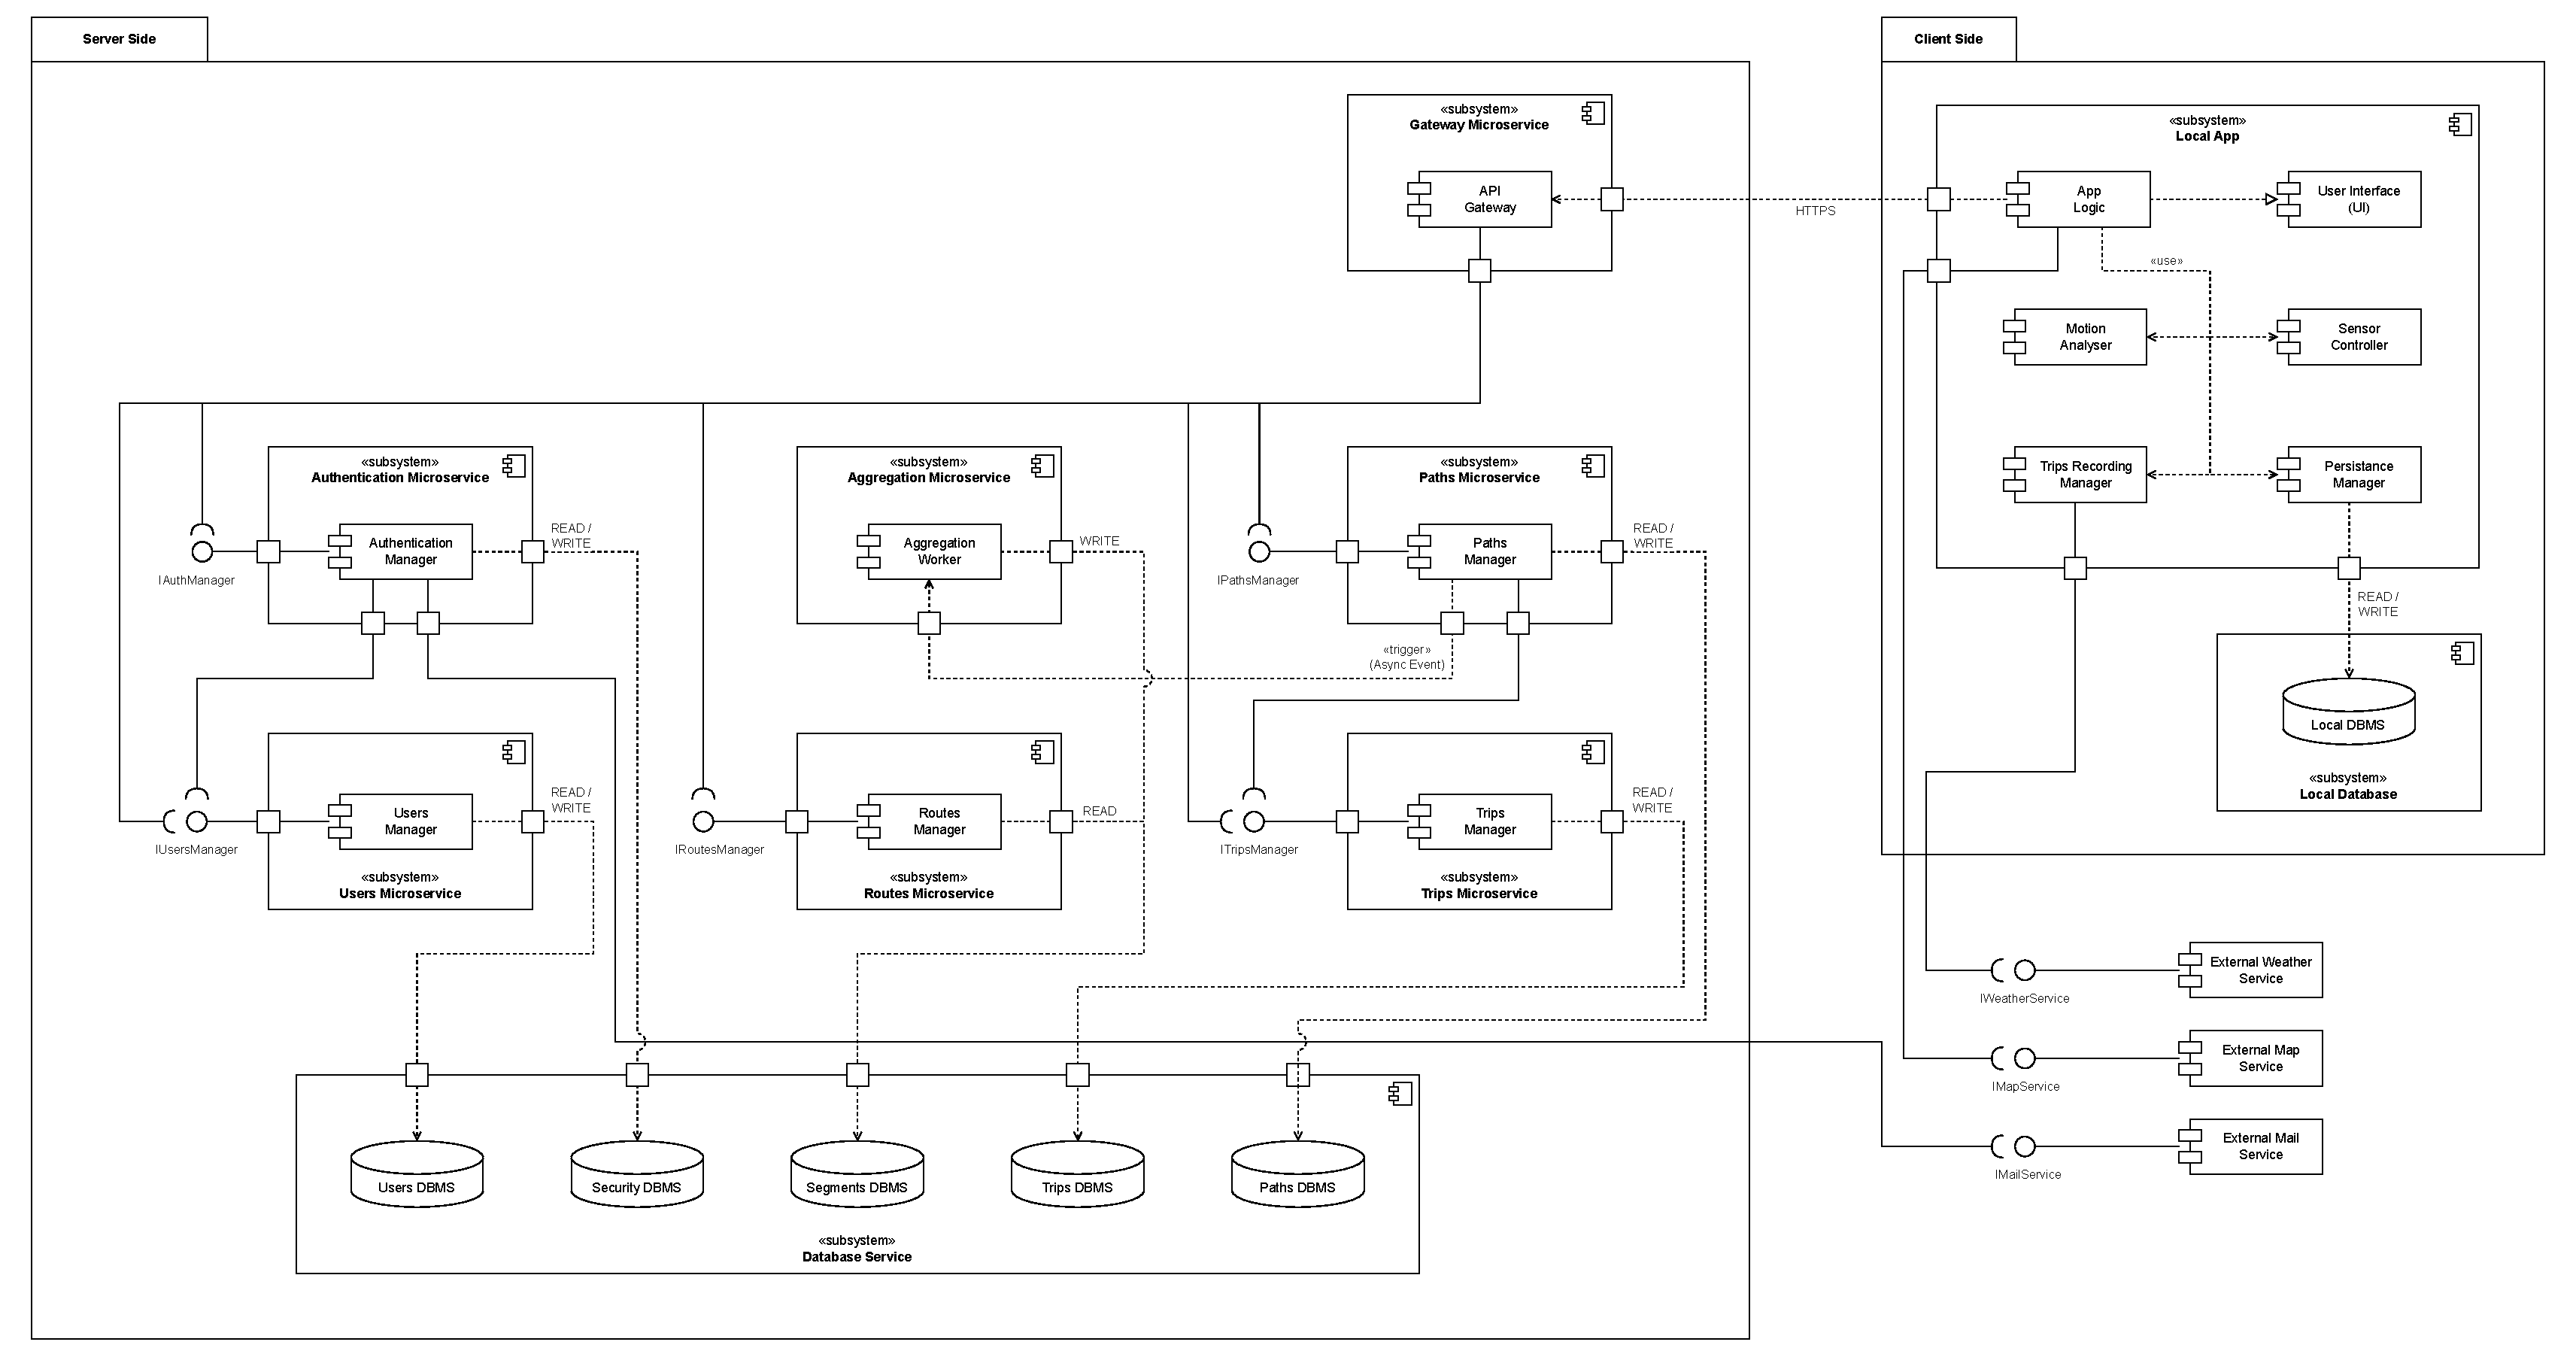
\includegraphics[width=\textwidth]{pdf/component_diagram.pdf}
    \caption{UML Components Diagram.}
    \label{fig:component_diagram}
\end{figure}

Please refer to Figure \ref{fig:appendix_component_diagram} (Page \pageref{fig:appendix_component_diagram}) for a bigger version.
\subsection{Components Descriptions}
The System architecture is divided into two main processing environments: the \emph{Client Side}, responsible for real-time data collection and local interactions, and the \emph{Server Side}, which handles data consolidation, synchronization, and global analytics.

\subsubsection*{Client Side Components}
The client application acts as a \emph{Thick Client}, designed to operate autonomously even in the absence of network connectivity (\eg, when recording a Trip in remote locations).
\begin{itemize}
    \item \textbf{Sensor Controller:} This component serves as the hardware abstraction layer. It interfaces directly with the device's physical sensors (GPS and Accelerometer) to retrieve raw telemetry data streams at high frequency.
    
    \item \textbf{Motion Analyzer:} A critical module for edge computing. It processes the raw data stream from the Sensor Controller locally to detect specific events (\eg, sudden braking, potholes, or surface irregularities) and compute real-time road quality metrics. This reduces the bandwidth usage by transmitting only processed insights rather than raw sensor noise.
    
    \item \textbf{Trips Recording Manager:} Orchestrates the active Trip session. It subscribes to the processed data from the Motion Analyzer, organizes it into a coherent Trip structure (associating timestamps and locations), and manages the start/stop/pause logic of a recording.
    
    \item \textbf{App Logic:} The central coordinator of the mobile application. It manages the application state, handles navigation between UI screens, and orchestrates communication with the backend.
    
    \item \textbf{Persistence Manager:} This component implements the \emph{Offline-First} pattern. It abstracts the underlying \emph{Local DBMS}, handling all read/write operations on the device. It ensures that Trip data is securely stored locally immediately after recording and manages the synchronization queue when the device regains connectivity. It also stores authentication data, such as JWTs.
    
    \item \textbf{Local DBMS:} A lightweight relational database (\eg, SQLite) residing on the User's device, used for caching Paths and storing unsynchronized Trips.
\end{itemize}

\subsubsection*{Server Side Components}
The backend is structured as a generic \emph{Microservices Architecture}, where functional domains are encapsulated in independent subsystems to ensure scalability and fault isolation.
\begin{itemize}
    \item \textbf{Gateway Microservice:}
    It acts as the single entry point for all client requests. It handles SSL termination, request routing, and load balancing, forwarding calls to the appropriate microservice interface (\eg, \texttt{IAuthManager}, \texttt{ITripsManager}).

    \item \textbf{Authentication \& User Microservices:}
    These subsystems handle the identity management (via the \texttt{Authentication Manager}) and User profile data (via the \texttt{Users Manager}), managing credentials and personal settings stored in their respective databases.

    \item \textbf{Trips Microservice:}
    Manages the lifecycle of Trip entities (temporal metadata). As depicted in the diagram, it has a functional dependency (\texttt{«use»}) on the \emph{Paths Microservice}: when a Trip is saved, the Trips Manager invokes the Paths Manager to persist the associated geospatial data.

    \item \textbf{Paths Microservice:}
    Responsible for the catalogue of Paths (CRUD operations). Crucially, upon modifying a Path's visibility, it triggers an asynchronous event (\texttt{«trigger»}) towards the \emph{Aggregation Worker} to initiate the map update process without blocking the User response.

    \item \textbf{Routes Microservice:}
    Dedicated to complex geospatial operations. It handles pathfinding queries and spatial searches, interacting with the geospatial data in the \emph{Segments DBMS}.

    \item \textbf{Aggregation Microservice:}
    A background processing unit responsible for maintaining the global map consistency. It does not expose any interfaces as it listens for change events. When triggered, it recalculates the scores of road segments by merging new User data with historical records.

    \item \textbf{Database Service:} The persistence layer groups the System's databases. While most microservices maintain exclusive ownership of their data (\eg, \emph{Trips DBMS}, \emph{Users DBMS}) to foster decoupling, the \emph{Segments DBMS} represents a notable exception. 
    It acts as a Shared Data Store accessed by multiple services (\texttt{Routes Manager} and \texttt{Aggregation Worker}). This design choice is driven by the specific requirement to perform heavy geospatial calculations (Routing) and global updates (Reliability Scoring) on the same dataset without the overhead of data duplication or continuous synchronization.
\end{itemize}

\subsubsection*{External Services}
The System relies on third-party providers to fulfill specific capabilities that are outside the core domain logic. These services are integrated via abstract interfaces to ensure modularity and avoid vendor lock-in.

\begin{itemize}
    \item \textbf{External Map Service:} Provides the fundamental geospatial infrastructure for the frontend. The Client Application consumes this service to render map tiles, perform geocoding operations, and support the User Interface during track visualization. The System is designed to support open solutions like \textbf{OpenStreetMap}\footnote{\url{https://www.openstreetmap.org/}} and \textbf{OpenCycleMap}\footnote{\url{https://www.opencyclemap.org/}}, as well as proprietary providers like \textbf{Google Maps Platform}, depending on the required licensing and tile resolution.

    \item \textbf{External Weather Service:} A third-party API used to enrich Trip data context. The Client Side interacts with this service to fetch environmental conditions (\eg, temperature, weather status) corresponding to the specific location and time of a recorded Trip. A standard provider for this capability is \textbf{OpenWeatherMap}\footnote{\url{https://openweathermap.org/}}, but the architecture supports any REST-compliant weather API (\eg, AccuWeather, WeatherAPI).

    \item \textbf{External Mail Service:} An infrastructure provider responsible for the delivery of transactional emails. It is invoked by the \textbf{Authentication Manager} to dispatch One-Time Passwords (OTP) during the User registration or password reset flows. Industry-standard SMTP providers such as \textbf{SendGrid}\footnote{\url{https://sendgrid.com/}} or \textbf{Mailgun}\footnote{\url{https://www.mailgun.com/}} are suitable candidates for high-deliverability requirements.
\end{itemize}

\section{Deployment View}

\subsection{Overview}
The Deployment View illustrates the mapping of software artifacts onto the physical hardware nodes. 
The \emph{Best Bike Paths} System adopts a distributed architecture to ensure scalability, fault tolerance, and offline capabilities. The physical topology is organized into a \textbf{3-Tier} structure (Client, Server, Data), which hosts the \textbf{6 Logical Layers} defined in the architectural design.

The deployment strategy relies heavily on containerization (Docker) and orchestration (Kubernetes) for the backend, while the client side is designed as a \emph{Thick Client} to perform local data processing and persistence.

\subsection{Deployment Diagram}
Figure \ref{fig:deployment_diagram} depicts the UML Deployment Diagram of the System. 
It highlights the nesting of execution environments, showing how the application logic is encapsulated within the mobile operating System on the client side, and within the Kubernetes cluster on the server side.\footnote{Inter-node connections are not shown to avoid readability issues, but please note that nodes can communicate via HTTP/gRPC protocol.}

\begin{figure}[H]
    \centering
    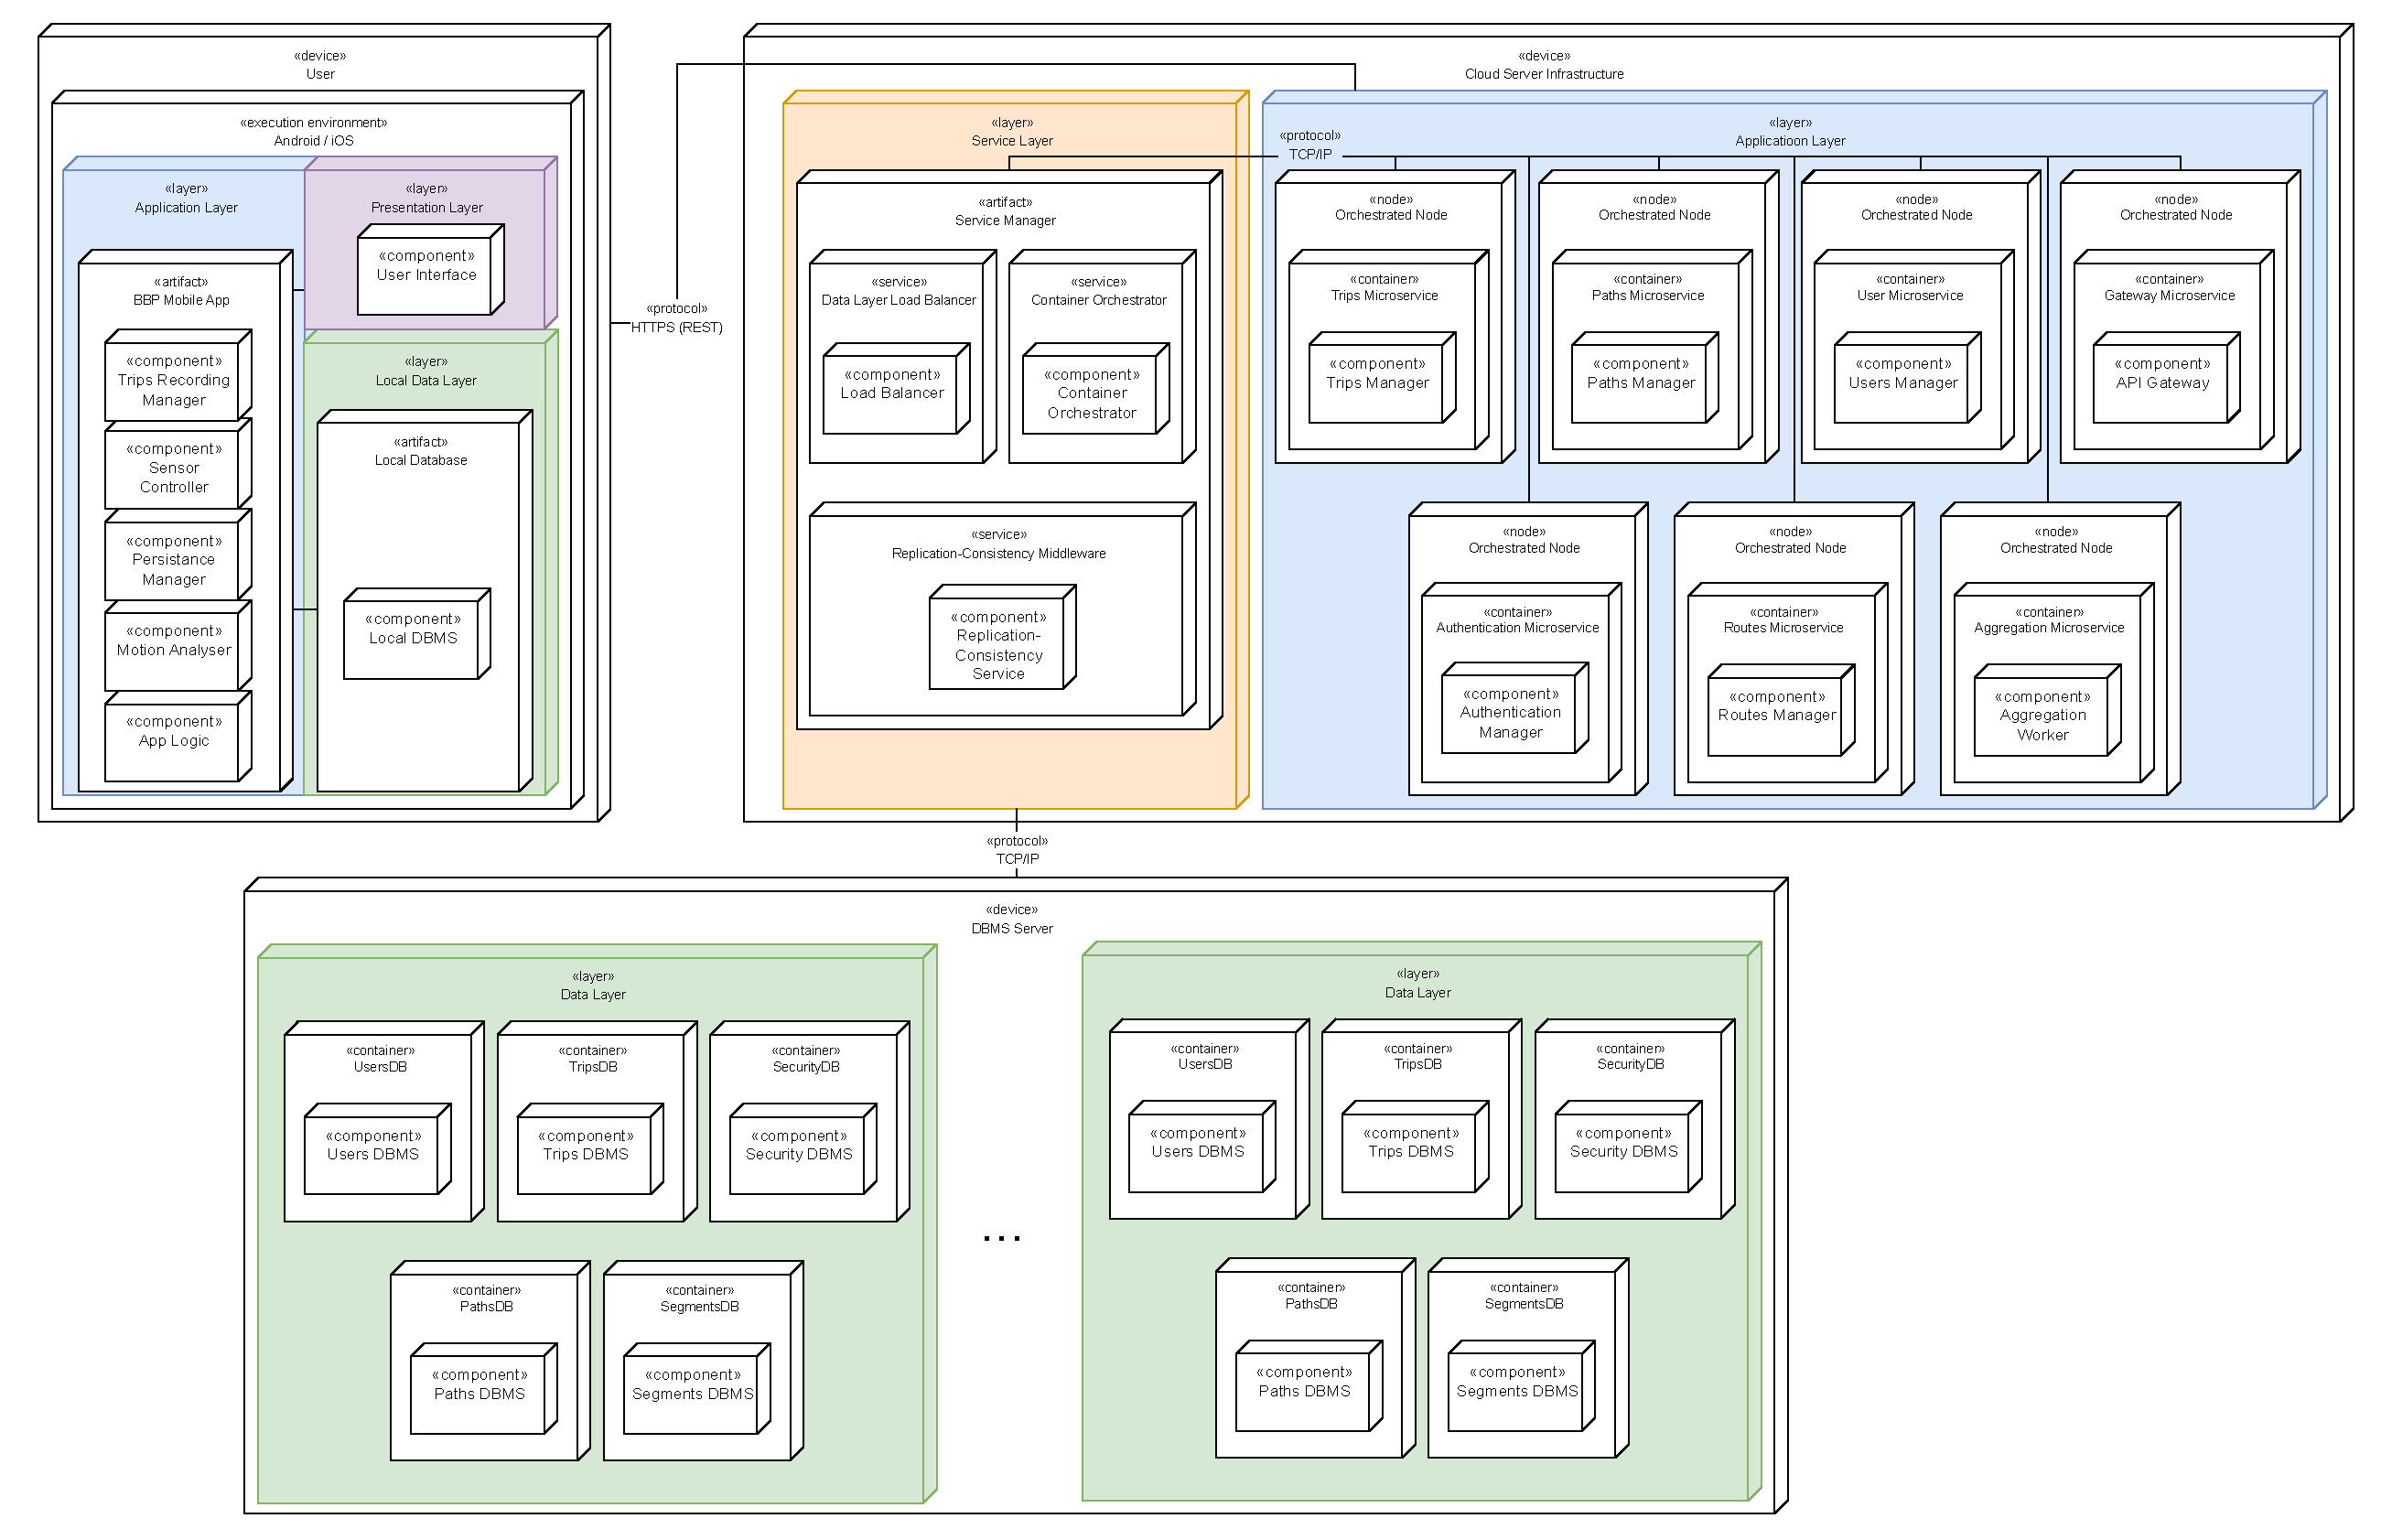
\includegraphics[width=\textwidth]{pdf/deployment_diagram.pdf}
    \caption{UML Deployment Diagram.}
    \label{fig:deployment_diagram}
\end{figure}

\noindent
Please refer to Figure \ref{fig:appendix_deployment_diagram} (Page \pageref{fig:appendix_deployment_diagram}) for a bigger version.

\subsection{Node mapping}
The following sections describe the specific configuration of each node and the software artifacts deployed on them.

\subsubsection*{Tier 1: User Client Device}
This node represents the end-User's smartphone. Given the \emph{Thick Client} nature of the application, this node bears a significant computational load.
\begin{itemize}
    \item \textbf{Hardware Node}: Smartphone (Android / iOS).
    \item \textbf{Execution Environment}: Mobile Operating System (Android OS or iOS).
    \item \textbf{Hosted Layers}:
    \begin{enumerate}
        \item \textbf{Presentation Layer}: Hosted within the Mobile App artifact, responsible for UI rendering.
        \item \textbf{Mobile Application Layer}: Hosted within the Mobile App artifact. It includes the \emph{Motion Analyzer} component for real-time sensor processing.
        \item \textbf{Client Data Layer}: Hosted within the \emph{Local Database} artifact. It ensures data persistence when the device is offline. A possible implementation might be through SQLite.
    \end{enumerate}
\end{itemize}

\subsubsection*{Tier 2: Backend Server Infrastructure}
This node represents the cloud infrastructure. It is abstracted by the orchestration layer, allowing the System to treat a cluster of physical machines as a single execution environment.
\begin{itemize}
    \item \textbf{Hardware Node}: Cloud Virtual Machines (Worker Nodes).
    \item \textbf{Execution Environment}: \textbf{Kubernetes Cluster} (Orchestration Layer).
    \item \textbf{Hosted Layers}:
    \begin{enumerate}
        \setcounter{enumi}{3} 
        \item \textbf{Server Application Layer}: Composed of Docker Containers (Pods) running the microservices (\emph{User Service}, \emph{Trip Service}, \emph{Path Service}, \emph{Routes Service}, \emph{Aggregation Worker}) and the API Gateway.
        \item \textbf{Service Orchestration Layer}: The Kubernetes control plane itself, managing the lifecycle and networking of the artifacts mentioned above.
    \end{enumerate}
\end{itemize}

\subsubsection*{Tier 3: Data Persistence Server}
To ensure data integrity and isolation, the primary database runs on a dedicated environment, separated from the application logic.
\begin{itemize}
    \item \textbf{Hardware Node}: Dedicated Database Server or Managed Cloud Database Instance.
    \item \textbf{Execution Environment}: PostgreSQL Engine.
    \item \textbf{Hosted Layers}:
    \begin{enumerate}
        \setcounter{enumi}{5} 
        \item \textbf{Server Data Layer}: Hosted within the \emph{Spatial DBMS} artifact (PostgreSQL + PostGIS extension). It stores the persistent state of the System (Users, Paths, Trips, Segments).
    \end{enumerate}
\end{itemize}

\subsection{Detailed Layer Decisions}
\subsubsection*{Client Logic and Local Persistence}
The decision to implement a \textbf{Thick Client} architecture with a dedicated \textbf{Client Data Layer} (SQLite) is driven by the "Offline-First" requirement. 
Instead of relying on a continuous network stream, the mobile application acts as a stand-alone unit during the Trip recording. 
\begin{itemize}
    \item \textbf{Local Pre-processing}: The \emph{Mobile Application Layer} processes high-frequency sensor data locally. Only aggregated events (\eg, detected potholes) and simplified Path coordinates are stored, significantly reducing bandwidth consumption.
    \item \textbf{Synchronization}: The local database acts as a temporary buffer. Data synchronization is deferred until a Trip ends and a stable connection is available.
\end{itemize}

\subsubsection*{API Gateway and Load Balancing}
To decouple the client from the internal microservices, an \textbf{API Gateway} has been introduced in the Server Application Layer.
\begin{itemize}
    \item \textbf{Unified Interface}: It exposes a stable, public API to the mobile clients, hiding the complexity of the internal microservices network.
    \item \textbf{Scalability}: The API Gateway is stateless. This allows the orchestration layer to \textbf{replicate} the Gateway across multiple pods. A load balancer distributes incoming traffic among these replicas, preventing the Gateway itself from becoming a bottleneck or a single point of failure.
\end{itemize}

\subsubsection*{Service Orchestration, Resiliency and Scalability}
The \textbf{Service Orchestration Layer} (Kubernetes) is the core enabler of the System's reliability. It manages the lifecycle of the Server Application Layer components through:
\begin{itemize}
    \item \textbf{Replication}: Critical services (such as the \emph{User Service} and \emph{Trip Service}) are deployed with a replication factor greater than one ($N \geq 2$). If one instance is busy or fails, traffic is seamlessly routed to the others.
    \item \textbf{Resiliency (Self-Healing)}: The orchestrator continuously monitors the health of the pods. If a microservice crashes (\eg, due to a runtime error), Kubernetes automatically restarts the container to restore the desired state without human intervention.
    \item \textbf{Horizontal Scalability}: The layer monitors resource usage (CPU/RAM). During peak traffic, it automatically provisions additional replicas of the stressed services (Autoscaling), ensuring consistent performance.
\end{itemize}

\subsubsection*{Server Data Layer Optimization}
For the \textbf{Server Data Layer}, the choice of a Spatial DBMS (PostgreSQL with PostGIS) is dictated by the domain efficiency.
Storing geospatial data as native geometric objects (Point, Linestring) allows the System to perform complex spatial queries (\eg, finding potholes within a radius) using optimized R-Tree indices, which is significantly faster than performing mathematical calculations at the application level.

\section{Component Interfaces}
\subsection{REST API Interface}

The interaction between the Client Tier and the Server Tier, as well as the communication among internal microservices, relies on a RESTful API architecture.
This section defines the structural patterns, addressing schemes, and the logical division between public and internal interfaces.

\subsubsection*{General Design Principles}
All APIs share the following technical characteristics to ensure consistency and interoperability:
\begin{itemize}
    \item \textbf{Protocol}: HTTPS (TLS 1.3) for public communication; HTTP/gRPC for internal cluster traffic.
    \item \textbf{Data Format}: JSON (JavaScript Object Notation) is used for all request bodies and response payloads.
    \item \textbf{Date Format}: ISO 8601 Strings (\eg, \texttt{2025-01-07T14:30:00Z}).
    \item \textbf{Error Handling}: Standard HTTP Status Codes (2xx for success, 3xx for redirects, 4xx for client errors, 5xx for server errors) accompanied by a JSON error object.
\end{itemize}

\subsubsection*{URI Structure and Namespaces}
The System distinguishes between APIs exposed to the outside world and APIs used strictly for inter-service communication.
\begin{description}
    \item[Public Interface Strategy]
    The public API is exposed via the \textbf{API Gateway}. It acts as the single entry point for the mobile application.
\begin{itemize}
    \item \textbf{Base Domain}: \texttt{https://api.bestbikePaths.com}
    \item \textbf{Versioning}: All public URIs are versioned to ensure backward compatibility.
    \item \textbf{Pattern}: \texttt{METHOD /api/v1/<resource>/...}
    \end{itemize}
    \item[Internal Interface Strategy]
    Internal APIs are accessible only within the Kubernetes cluster private network. They are not reachable from the public internet.
\begin{itemize}
    \item \textbf{Purpose}: These endpoints allow microservices to exchange data or trigger actions (\eg, Auth Service telling User Service to create a profile) without exposing these operations to the client.
    \item \textbf{Pattern}: \texttt{METHOD /internal/<service-name>/<action>}

\end{itemize}
\end{description}


\subsubsection*{API Macro Areas}
The API resources are organized into logical macro-areas corresponding to the underlying microservices domain\footnote{Note that the \emph{Aggregation Worker} does not expose any API as it works by listening to events.}:

\begin{itemize}
    \item \texttt{/auth}: Manages registration, login, OTP verification, and token refresh.
    \item \texttt{/users}: Handles User profiles, settings, and personal statistics.
    \item \texttt{/trips}: Manages Trip recording, upload, and history retrieval.
    \item \texttt{/paths}: Handles the retrieval of map segments, tiles, and pothole data.
    \item \texttt{/routes}: Manages Pathfinding operations, calculating optimal routes based on distance and road safety scores.
\end{itemize}

\subsection{Public API Endpoints (Gateway)}
The following tables detail the REST interface exposed by the API Gateway.\footnote{Note on Status Codes: Standard technical errors (\eg, \emph{500 Internal Server Error}) and generic authorization errors (\eg, \emph{401 Unauthorized}) are omitted from the tables. All endpoints assume a valid JWT token in the \texttt{Authorization} header unless stated otherwise.}

All URIs listed below are relative to the base path: \textbf{\texttt{/api/v1}}.

% --- AUTHENTICATION ---
\subsubsection*{Authentication (Prefix: \texttt{/auth})}
\begin{table}[H]
    \sf
    \small
    \centering
    \renewcommand{\arraystretch}{1.5}
    \begin{tabularx}{\textwidth}{|l|p{2.5cm}|p{4cm}|X|}
    \hline
    \rowcolor{lightgray} \textbf{Method} & \textbf{URI} & \textbf{Request Payload / Query} & \textbf{Response} \\ \hline

    \texttt{POST} & \texttt{/signup} & 
    \textbf{Payload:} \newline \texttt{\{ "email": "...",\newline  "password": "...",\newline  "userData": \{...\} \}} \newline \textbf{Query:} \newline \textit{None} & 
    \textbf{200 OK}: OTP sent to email. \newline 
    \textbf{409 Conflict}: Email already registered. \\ \hline

    \texttt{POST} & \texttt{/verify-otp} & 
    \textbf{Payload:} \newline \texttt{\{ "email": "...",\newline  "code": "..." \}} \newline \textbf{Query:} \newline \textit{None} & 
    \textbf{201 Created}: \newline \texttt{\{ "token": "JWT...",\newline  "userId": "..." \}} \newline 
    \textbf{400 Bad Request}: Invalid code. \\ \hline

    \texttt{POST} & \texttt{/login} & 
    \textbf{Payload:} \newline \texttt{\{ "email": "...",\newline  "password": "..." \}} \newline \textbf{Query:} \newline \textit{None} & 
    \textbf{200 OK}: \newline \texttt{\{ "token": "JWT...",\newline  "userId": "..." \}} \newline 
    \textbf{401 Unauthorized}: Invalid credentials. \\ \hline
    
    \texttt{POST} & \texttt{/guest-token} & 
    \textbf{Payload:} \newline \texttt{\{ "deviceId": \newline "uuid..." \}} \newline \textbf{Query:} \newline \textit{None} & 
    \textbf{200 OK}: \newline \texttt{\{ "token": "GuestJWT...",\newline "expiresIn": "..." \}} \\ \hline
    \end{tabularx}
    \caption{Public API - Authentication}
    \label{tab:api_public_auth}
\end{table}

% --- TRIPS ---
\subsubsection*{Trips (Prefix: \texttt{/trips})}
\begin{table}[H]
    \sf
    \small
    \centering
    \renewcommand{\arraystretch}{1.5}
    \begin{tabularx}{\textwidth}{|l|p{2.5cm}|p{4cm}|X|}
    \hline
    \rowcolor{lightgray}\textbf{Method} & \textbf{URI} & \textbf{Request Payload / Query} & \textbf{Response} \\ \hline
    
    \texttt{POST} & \texttt{/save} & \textbf{Payload:} \newline \texttt{\{ "tripData": \{...\},\newline "geometry": \{...\}, \newline "visibility": \newline "PUBLIC"|"PRIVATE" \}} \newline \textbf{Query:} \newline \textit{None} & 
    \textbf{201 Created}:\newline \texttt{\{ "tripId": "..." \}} \newline
    \textbf{400 Bad Request}: Invalid format. \\ \hline
    
    \texttt{DELETE} & \texttt{/\{id\}} &
    \textbf{Payload:} \newline \textit{None} \newline \textbf{Query:} \newline
    \texttt{?cascade=true|false} & 
    \textbf{204 No Content}: Deleted. \newline
    \textbf{403 Forbidden}: Not owner. \newline
    \textbf{404 Not Found}: Trip ID invalid. \\ \hline
    
    \texttt{GET} & \texttt{/list} &
    \textbf{Payload:} \newline \textit{None} \newline \textbf{Query:} \newline
    \texttt{?page=...\&limit=...} & 
    \textbf{200 OK}: \newline \texttt{\{ "trips": [ \{ ... \} ], \newline "total": "..." \}} \\ \hline
    
    \texttt{GET} & \texttt{/\{id\}} & 
    \textbf{Payload:} \newline \textit{None} \newline \textbf{Query:} \newline \textit{None} & 
    \textbf{200 OK}:\newline 
    \texttt{\{ "tripData": \{...\},\newline "geometry": \{...\}\}} \newline
    \textbf{404 Not Found}: Invalid ID. \newline
    \textbf{403 Forbidden}: Not owner. \\ \hline
    \end{tabularx}
    \caption{Public API - Trips}
    \label{tab:api_public_trips}
\end{table}

% --- PATHS ---
\subsubsection*{Paths (Prefix: \texttt{/paths})}
\begin{table}[H]
    \sf
    \small
    \centering
    \renewcommand{\arraystretch}{1.5}
    \begin{tabularx}{\textwidth}{|l|p{2.5cm}|p{4cm}|X|}
    \hline
    \rowcolor{lightgray}\textbf{Method} & \textbf{URI} & \textbf{Request Payload / Query} & \textbf{Response} \\ \hline
    
    \texttt{POST} & \texttt{/save} & 
    \textbf{Payload:} \newline \texttt{\{ "geometry": \{...\}, \newline "visibility": \newline "PUBLIC"|"PRIVATE" \}} \newline \textbf{Query:} \newline \textit{None} & 
    \textbf{201 Created}: \newline \texttt{\{ "pathId": "..." \}} \newline
    \textbf{400 Bad Request}: Invalid geometry format. \\ \hline
    
    \texttt{DELETE} & \texttt{/\{id\}} & 
    \textbf{Payload:} \newline \textit{None} \newline \textbf{Query:} \newline \textit{None} & 
    \textbf{204 No Content}: Deleted. \newline
    \textbf{409 Conflict}: Linked to a Trip. \newline
    \textbf{404 Not Found}: Invalid ID. \newline
    \textbf{403 Forbidden}: Not owner. \\ \hline
    
    \texttt{POST} & \texttt{/\{id\}/chg-vis} & 
    \textbf{Payload:} \newline \texttt{\{ "visibility": \newline "PUBLIC"|"PRIVATE" \}} \newline \textbf{Query:} \newline \textit{None} & 
    \textbf{200 OK}: Status updated. \newline
    \textbf{403 Forbidden}: Not owner. \newline
    \textbf{404 Not Found}: Path ID invalid. \\ \hline
    
    \texttt{GET} & \texttt{/list} & 
    \textbf{Payload:} \newline \textit{None} \newline \textbf{Query:} \newline \texttt{?page=...\&limit=...} & 
    \textbf{200 OK}: List of User's Paths. \\ \hline
    
    \texttt{GET} & \texttt{/\{id\}} & 
    \textbf{Payload:} \newline \textit{None} \newline \textbf{Query:} \newline \textit{None} & 
    \textbf{200 OK}: 
    \texttt{\{ "geometry": \{...\}, \newline "visibility": \newline "PUBLIC"|"PRIVATE" \}} \newline
    \textbf{404 Not Found}: Invalid ID. \newline
    \textbf{403 Forbidden}: Not owner. \\ \hline
    \end{tabularx}
    \caption{Public API - Paths}
    \label{tab:api_public_paths}
\end{table}

% --- ROUTES ---
\subsubsection*{Routes (Prefix: \texttt{/routes})}
\begin{table}[H]
    \sf
    \small
    \centering
    \renewcommand{\arraystretch}{1.5}
    \begin{tabularx}{\textwidth}{|l|p{2.5cm}|p{4cm}|X|}
    \hline
    \rowcolor{lightgray}\textbf{Method} & \textbf{URI} & \textbf{Request Payload / Query} & \textbf{Response} \\ \hline
    
    \texttt{GET} & \texttt{/calculate} & 
    \textbf{Payload:} \newline \textit{None} \newline \textbf{Query:} \newline \texttt{?start=lat,lon \& \newline end=lat,lon} & 
    \textbf{200 OK}: \newline \texttt{[ \{ "routeId": "...", \newline "segments": [...],\newline "score": "..." \} ]} \newline
    \textbf{404 Not Found}: No route found. \\ \hline
    \end{tabularx}
    \caption{Public API - Routing}
    \label{tab:api_public_routes}
    \end{table}
    
% --- USERS ---
\subsubsection*{Users (Prefix: \texttt{/users})}
\begin{table}[H]
    \sf
    \small
    \centering
    \renewcommand{\arraystretch}{1.5}
    \begin{tabularx}{\textwidth}{|l|p{2.5cm}|p{4cm}|X|}
    \hline
    \rowcolor{lightgray} \textbf{Method} & \textbf{URI} & \textbf{Request Payload / Query} & \textbf{Response} \\ \hline
    
    \texttt{GET} & \texttt{/\{id\}/profile} &
    \textbf{Payload:} \newline \textit{None} \newline \textbf{Query:} \newline \textit{None} & 
    \textbf{200 OK}:\newline \texttt{\{ "userData": \{...\}, \newline"stats": \{...\} \}} \newline
    \textbf{404 Not Found}: User ID not found. \newline
    \textbf{403 Forbidden}: Mismatch owner/caller. \\ \hline
    \end{tabularx}
    \caption{Public API - Users}
    \label{tab:api_public_users}
\end{table}


\subsubsection{Internal Microservices Interfaces}
Most internal endpoints managed by the API Gateway mirror the Public API definitions with a 1:1 mapping, simply forwarded to the respective microservice within the cluster (\eg, \texttt{/internal/auth/login} accepts the same payload as the public counterpart).

However, specific endpoints exist solely for \textbf{Inter-Service Communication} to support business transactions that span multiple domains. These are detailed below.

For the sake of clarity and uniformity with the Public API documentation, the interfaces below are described using logical REST-like resource paths. However, in the actual deployment, these high-frequency internal interactions are implemented using \textbf{gRPC} (over HTTP/2) and \textbf{Protocol Buffers} to minimize latency and serialization overhead.

\begin{table}[H]
\sf
\small
\centering
\renewcommand{\arraystretch}{1.5}
\begin{tabularx}{\textwidth}{|l|l|l|X|}
\hline
\rowcolor{lightgray} \textbf{Target Service} & \textbf{Method \& URI} & \textbf{Caller} & \textbf{Payload / Response} \\ \hline

\textbf{Users Manager} & \texttt{POST /create} & 
\textbf{Auth Service} & 
\textbf{In:} \texttt{\{ "userId": "...", \newline "email": "...", \newline "name": "..." \}} \newline
\textbf{Out:} 201 Created \\ \hline


\textbf{Paths Manager} & \texttt{GET /\{id\}/geometry} & 
\textbf{Aggregation Worker} & 
\textbf{In:} \textit{None (GET)} \newline
\textbf{Out:} 200 OK \newline \texttt{\{ "geometry": \{...\}, \newline "metadata": \{...\} \}} \\ \hline

\textbf{Paths Manager} & \texttt{DELETE /\{id\}} & 
\textbf{Trips Service} & 
\textbf{In:} \textit{None} \newline
\textbf{Out:} 204 No Content \\ \hline

\textbf{Paths Manager} & \texttt{PATCH /\{id\}} & 
\textbf{Trips Service} & 
\textbf{In:} \texttt{\{ "tripId": null \}} \newline
\textbf{Out:} 200 OK \\ \hline

\end{tabularx}
\caption{Internal Inter-Service APIs}
\label{tab:api_internal_services}
\end{table}

\subsection{External Service Interfaces}
\label{subsubsec:ESI}
The System relies on third-party services to fulfil specific capabilities. The following table summarizes the external contracts consumed by both the Mobile Client and the Backend Microservices.


To maintain flexibility and avoid \emph{vendor lock-in}, the interfaces described below are defined as \emph{logical abstractions}. Their use in the sequence diagrams are an example of a possible implementation. The \emph{Adapter Design Pattern} can be used to eventually translate calls.

\begin{table}[H]
\sf
\small
\centering
\renewcommand{\arraystretch}{1.5}
\begin{tabularx}{\textwidth}{|l|l|X|X|}
\hline
\rowcolor{lightgray} \textbf{External Service} & \textbf{Consumer} & \textbf{Purpose} & \textbf{Data Exchanged} \\ \hline

\textbf{Map Service} & 
\textbf{Client App} & 
Rendering map tiles and Geocoding addresses. & 
\textbf{Out:} Address string or Tile Coordinates (x,y,z). \newline
\textbf{In:} Lat/Lon coordinates or PNG Tile images. \\ \hline

\textbf{Email Provider} & 
\textbf{Auth Service} & 
Sending OTP codes for 2FA and account verification. & 
\textbf{Out:} Recipient Email, OTP Code, Template ID. \newline
\textbf{In:} Delivery Status. \\ \hline

\textbf{Weather Service} & 
\textbf{Trip Manager} & 
Enriching Trip data with weather conditions. & 
\textbf{Out:} Lat/Lon, Timestamp. \newline
\textbf{In:} Temperature, Condition (Rain/Sun), Humidity. \\ \hline
\end{tabularx}
\caption{External Service Interfaces}
\label{tab:api_external}
\end{table}

\newpage

\section{Runtime View}
What follow are the ten Sequence Diagrams corresponding to the ten Use Cases illustrated in the RASD. A bigger version of the diagrams is available in the \hyperref[sec:appendix_diagrams]{Appendix} to this document.

\subsubsection*{[SD1] Sign Up by a User}
The sequence diagram illustrates the registration process for an Unregistered User, enforcing a secure two-step verification flow. The interaction begins with the User inputting their credentials via the \emph{User Interface}. The \emph{App Logic} first performs local validation on the input fields; upon success, it transmits the request through the \emph{API Gateway} to the \emph{Authentication Service}. This service queries the \emph{SecurityDBMS} to verify the uniqueness of the provided email. If the email is available, a new record with a \texttt{PENDING} status is created, and the \emph{EmailProvider} is triggered to dispatch a One-Time Password (OTP) to the User.

In the second phase, the User submits the received OTP for verification. The \emph{Authentication Service} validates the code against the \emph{SecurityDBMS}. Upon successful validation, the account status is updated to \texttt{ACTIVE}. To ensure separation of concerns, the \emph{Authentication Service} subsequently invokes the \emph{Users Manager} via an internal API to initialize the User's persistent profile in the \emph{UsersDBMS}. Finally, a JWT is generated and returned to the \emph{App Logic}, which locally persists the session token and redirects the User to the application dashboard.

\begin{figure}[hp]
    \centering
    \includesvg[width=\textwidth, inkscapelatex=false]{figures/sd1.svg}
    \caption{SD1. Sign Up by a User}
    \label{fig:SD1}
\end{figure}
\newpage
\subsubsection*{[SD2] Log In by a User}
The diagram details the authentication procedure for a Registered User, which involves both credential verification and the initialization of the local application context. The process initiates with the User submitting their email and password via the \emph{User Interface}. Following a local format validation by the \emph{App Logic}, the credentials are transmitted through the \emph{API Gateway} to the \emph{Authentication Service}. This component retrieves the stored password hash and account status from the \emph{SecurityDBMS} to perform a cryptographic verification. Upon success, the service generates a JWT pair, which is returned to the client and persisted in the device's secure storage.

Subsequently, to satisfy the System's Thick Client architectural requirements, the \emph{App Logic} automatically triggers a data synchronization routine. It requests the User's full profile details using the newly acquired access token. The \emph{API Gateway} routes this request to the \emph{Users Manager}, which queries the \emph{UsersDBMS} for personal attributes, preferences, and statistics. This payload is downloaded and cached in the local SQLite database, ensuring the application is immediately functional, even in potential offline scenarios, before finally redirecting the User to the main dashboard.

\vspace{1cm}
\begin{figure}[H]
    \centering
    \includesvg[width=\textwidth, inkscapelatex=false]{figures/sd2.svg}
    \caption{SD2. Log In by a User}
    \label{fig:SD2}
\end{figure}
\newpage
\subsubsection*{[SD3] Access as Guest}
The sequence outlines the procedure for granting limited access to an Unregistered User via an anonymous session. The process is triggered by the User selecting the Guest option on the \emph{User Interface}. The \emph{App Logic} initiates a request to the \emph{API Gateway}, which forwards the call to the \emph{Authentication Service}. Unlike standard authentication, this service does not query the User database; instead, it generates an ephemeral JWT with restricted privileges (Guest Role), valid for a limited duration, and returns it to the client.

Upon receiving the token, the \emph{App Logic} securely stores it for subsequent read-only API calls. Crucially, to maintain architectural consistency with the Registered User flow, the System instantiates a placeholder profile within the local SQLite database. This allows the application to maintain a persistent link at further openings.
\vspace{1cm}
\begin{figure}[H]
    \centering
    \includesvg[width=\textwidth, inkscapelatex=false]{figures/sd3.svg}
    \caption{SD3. Access as Guest}
    \label{fig:SD3}
\end{figure}
\newpage
\subsubsection*{[SD4] Record a Trip}
The diagram demonstrates the core offline capability of the System, detailing how a Trip is recorded using strictly local resources while attempting to enrich data when connectivity permits. The process begins with the Registered User initiating the recording via the \emph{User Interface}. The \emph{Trip Recording Manager} instantiates a new session object and commands the \emph{Sensor Controller} to activate the GPS, accelerometer, and gyroscope hardware at high frequency to ensure granular data capture.

During the active recording phase, the System operates in a continuous sampling loop. Incoming raw sensor data is routed to the \emph{Motion Analyser}, which performs edge computing tasks such as noise filtering and motion state detection. If the User is stationary, the System triggers the \emph{Smart Pause} logic to suspend the timer. Conversely, when motion is detected, the \emph{Trip Recording Manager} updates the Trip statistics, checks for potential anomalies (\eg, potholes), and buffers the data points in memory.

Upon termination, the System disables the sensors to conserve battery. Before final persistence, the logic attempts to retrieve environmental context by querying an external \emph{Weather Service} using the last known GPS coordinates. This interaction is designed to be non-blocking: if the API is reachable, metadata are retrieved; otherwise, in case of timeout or connectivity errors or unavailability, the weather data is simply omitted. Finally, the \emph{Trip Recording Manager} flushes the buffered data, including the Path, statistics, anomalies, and any optional weather information, to the \emph{Local SQLite DB}, ensuring persistence before displaying the summary to the User.
\begin{figure}[hp]
    \centering
    \includesvg[width=\textwidth, inkscapelatex=false]{figures/sd4.svg}
    \caption{SD4. Record a Trip}
    \label{fig:SD4}
\end{figure}
\newpage
\subsubsection*{[SD5] Validate a Trip and a Path}
This sequence diagram depicts the final validation and persistence process of a \emph{Trip} and its associated \emph{Path} at the end of a recording session.
Consistent with the System's \emph{Thick Client} architecture and \emph{Offline-First} approach, the initial validation phase where the User confirms obstacles and defines the Path status is performed locally within the \emph{App Logic} without interacting with the backend.

Once the User confirms the save operation, the \emph{App Logic} transmits the complete payload (including Trip metadata, Path geometry, and validated obstacles) via the \emph{API Gateway} to the \emph{Trips Manager}. This service acts as the orchestrator for the transaction: it first persists the temporal metadata (\eg, duration, average speed) into the \emph{Trips DBMS}, and then synchronously invokes the \emph{Paths Manager} to handle the geospatial data storage in the \emph{Paths DBMS}.

If the User sets the Path visibility to \emph{Public}, the process triggers an asynchronous consistency mechanism. The \emph{Paths Manager} notifies the \emph{Aggregation Worker}, which runs in the background to retrieve historical data, merge it with the new contribution, and update the \emph{Score} of the affected road segments in the global map. This ensures that the User receives immediate confirmation of the saved Trip, while the computationally expensive aggregation task is handled separately.

\vspace{1cm}
\begin{figure}[hp]
    \centering
    \includesvg[width=\textwidth, inkscapelatex=false]{figures/sd5.svg}
    \caption{SD5. Validate a Trip and a Path}
    \label{fig:SD5}
\end{figure}
\newpage
\subsubsection*{[SD6] Change Path's visibility}
This sequence diagram illustrates the process of modifying the visibility status of an existing Path (\eg, switching from \emph{Private} to \emph{Public} or vice versa).

When the User toggles the visibility setting via the \emph{User Interface}, the \emph{App Logic} forwards the request to the \emph{Paths Manager} through the \emph{API Gateway}. The manager synchronously updates the Path's metadata in the \emph{Paths DBMS} to reflect the new state.

Crucially, this operation triggers a background consistency mechanism to ensure the global map remains accurate. Immediately after the local update, the \emph{Paths Manager} sends an asynchronous notification to the \emph{Aggregation Worker}. Depending on the new visibility state, the worker adjusts the global statistics: if set to \emph{Public}, the worker integrates the Path's segments statuses in the corresponding public road segments by the algorithm, valuing freshness and confirming reports; conversely, if set to \emph{Private}, it removes the Path's contribution and computes a new status based on history. This asynchronous design pattern allows the System to provide immediate feedback to the User (\emph{Visibility Updated}) while the computationally intensive map re-aggregation is performed by the worker in the background.

\vspace{1cm}
\begin{figure}[hp]
    \centering
    \includesvg[width=\textwidth, inkscapelatex=false]{figures/sd6.svg}
    \caption{SD6. Change Path's visibility}
    \label{fig:SD6}
\end{figure}
\newpage
\subsubsection*{[SD7] Create a Path manually}
The diagram depicts the flow for manually defining a new route without recording a live Trip. The process initiates with the Registered User interacting with the \emph{User Interface}, which first retrieves map tiles and road geometry from the \emph{Map Service} (\eg, via snapping APIs) to render the interface. The User iteratively defines the track geometry and attributes via the \emph{App Logic}. Upon confirmation, the \emph{App Logic} transmits the data through the \emph{API Gateway} to the \emph{Paths Manager}.

This component validates the geospatial consistency of the segments; if the data is valid, it persists the new Path in the \emph{Paths DBMS}. In accordance with the System's data quality requirements, if the Path's visibility is set to \emph{Public}, the \emph{Paths Manager} emits an event to the \emph{Aggregation Worker}. This worker retrieves the geometry via the internal API, calculates the scores of the affected road segments, and updates the \emph{Segments DBMS} to reflect the User's contribution on the global map.
\vspace{1cm}
\begin{figure}[H]
    \centering
    \includesvg[width=\textwidth, inkscapelatex=false]{figures/sd7.svg}
    \caption{SD7. Create a Path Manually}
    \label{fig:SD7}
\end{figure}

\newpage
\subsubsection*{[SD8] Search for a Route}
This sequence diagram outlines the workflow when a User searches for suitable Paths based on specific criteria (\eg, location, status, or length).

The process begins with the User submitting the search parameters via the \emph{User Interface}. The \emph{App Logic} forwards the query through the \emph{API Gateway} to the \emph{Routes Manager}. This component is responsible for handling geospatial queries: it accesses the \emph{Segments DBMS} to identify routes that match the User's requirements.

Once the matching items are retrieved, the \emph{Routes Manager} aggregates the results and returns a list of candidate routes to the \emph{App Logic}, which displays them to the User.
\vspace{1cm}

\begin{figure}[H]
    \centering
    \includesvg[width=\textwidth, inkscapelatex=false]{figures/sd8.svg}
    \caption{SD8. Search for a Route}
    \label{fig:SD8}
\end{figure}

\newpage
\subsubsection*{[SD9] Delete a Trip}
The diagram illustrates the interaction flow when a Registered User initiates the deletion of a recorded Trip. The process begins at the \emph{User Interface} layer, which prompts the User to specify the scope of the deletion: removing only the Trip statistics (keeping the Path as a manual entry) or deleting both the Trip and its associated geographical Path. The \emph{App Logic} forwards the request to the \emph{API Gateway}, which orchestrates the necessary calls to the \emph{Trips Manager}.


In both scenarios, the \emph{Trips Manager} performs a hard delete of the temporal metadata from the \emph{Trips DBMS}. If the User opts to delete both entities, the \emph{Trips Manager} invokes the \emph{Paths Manager} via the internal API. Crucially, if the Path was \emph{Public}, the \emph{Paths Manager} triggers the \emph{Aggregation Worker} (passing the geometry in the deletion event) to remove the User's contribution from the global road segment scores, ensuring data consistency.
\vspace{1cm}
\begin{figure}[H]
    \centering
    \includesvg[width=\textwidth, inkscapelatex=false]{figures/sd9.svg}
    \caption{SD9. Delete a Trip}
    \label{fig:SD9}
\end{figure}

\newpage
\subsubsection*{[SD10] Delete a Path}
The sequence depicts the control flow for the permanent removal of a User-defined Path. The process is initiated by the User via the \emph{User Interface} and mediated by the \emph{App Logic} and \emph{API Gateway}. Before proceeding with deletion, the \emph{Paths Manager} performs a critical dependency check on its local \emph{Paths DBMS} to ensure referential integrity: it verifies whether the Path is currently linked to an existing Trip (via the \texttt{trip\_id} foreign key). If dependencies are found, the operation is aborted, and a conflict error is returned to the User.

Conversely, if the Path is an orphan or manually created, the \emph{Paths Manager} proceeds with the deletion. As with the Trip deletion process, if the Path is \emph{Public}, the \emph{Paths Manager} asynchronously emits an event to the \emph{Aggregation Worker}. The worker then recalculates the scores of the affected road segments, removing the User's influence from the aggregated community data.
\vspace{1cm}
\begin{figure}[H]
    \centering
    \includesvg[width=\textwidth, inkscapelatex=false]{figures/sd10.svg}
    \caption{SD10. Delete a Path}
    \label{fig:SD10}
\end{figure}

\newpage
\section{Selected Architectural Styles and Patterns}
\label{sec:architectural_styles}
To address the complexity of the domain and the conflicting requirements of high availability and processing power, the System integrates several well-established architectural patterns.

\subsection*{Microservices and Database-per-Service}
The backend adopts a \textbf{Microservices Architecture} to ensure loose coupling and independent scalability. Adhering to the \emph{Database-per-Service} pattern, most services (Users, Trips, Auth) maintain exclusive ownership of their private databases. This prevents tight coupling and \emph{integration via database}, allowing each team to evolve their schema independently.

\paragraph*{CQRS (Command Query Responsibility Segregation)}
A strategic deviation from the strict Database-per-Service pattern is applied to the Geospatial Domain to solve the \emph{Read vs. Write} performance tension.
\begin{itemize}
    \item \textbf{Command Side (Write):} The \emph{Aggregation Worker} processes high-volume updates (Write Model) triggered by Users' contributions. It validates and merges data into the \emph{Segments DBMS}.
    \item \textbf{Query Side (Read):} The \emph{Routes Manager} (Read Model) accesses the same dataset but optimized for read-heavy operations (Pathfinding).
\end{itemize}
This separation allows the System to scale the worker nodes (for heavy processing) independently from the routing nodes (for low-latency queries).

\subsection*{Event-Driven Architecture (Pub/Sub)}
To handle long-running tasks without blocking the User Interface, the System implements an asynchronous \textbf{Publish/Subscribe} pattern.
When a synchronous action completes (\eg, \texttt{Path Saved} or \texttt{Visibility Changed}), the \emph{Paths Manager} publishes an event to a message broker. The \emph{Aggregation Worker}, acting as a subscriber, picks up the message and performs the recalculation in the background. This ensures the API remains responsive (low latency) while ensuring eventual consistency of the global map.

\subsection*{API Gateway (BFF Pattern)}
The \textbf{API Gateway} acts as a specialized entry point for the mobile application, implementing the \emph{Backend-for-Frontend (BFF)} pattern. It abstracts the complexity of the internal microservices mesh, providing a single, unified interface to the client. It handles cross-cutting concerns such as:
\begin{itemize}
    \item \textbf{Protocol Translation:} converting external HTTPS requests into internal gRPC calls.
    \item \textbf{Offloading:} handling SSL termination and Authentication verification.
    \item \textbf{Routing:} dispatching requests to the appropriate service instance.
\end{itemize}

\subsection*{Client-Side Patterns}
\begin{itemize}
    \item \textbf{Thick Client:} The mobile application is not a passive view but a computational node. It executes business logic (Motion Analysis) and data validation locally.
    \item \textbf{Offline-First:} The application is designed to function primarily offline during Trip recording. The \emph{Local Persistence Manager} acts as the source of truth for the UI, synchronizing with the server only when network conditions permit (Store-and-Forward).
\end{itemize}

\subsection*{Resiliency and Structural Patterns}
\begin{itemize}
    \item \textbf{Circuit Breaker:} To prevent cascading failures, a Circuit Breaker pattern is implemented in the API Gateway and inter-service calls. If a microservice (\eg, the \emph{Weather Service}) becomes unresponsive or exhibits high latency, the breaker \emph{opens}, immediately returning a fallback response (or cached data) instead of waiting for a timeout.
    \item \textbf{Adapter Pattern:} As described in Section \ref{subsubsec:ESI}, interaction with external providers (Maps, Weather, Email) is mediated by Adapters. This structural pattern encapsulates the specific API implementation of a vendor (\eg, Google Maps) behind a generic interface (\eg, \texttt{IMapService}). This ensures that switching providers does not require refactoring the core domain logic.
\end{itemize}

\section{Other Design Decisions}

\subsection*{Security and Data Privacy}
Given the sensitivity of location data, security is a foundational aspect of the design, addressing data at rest, data in transit, and access control.

Concerning Authentication and Authorization, the System employs \textbf{Stateless Authentication} via JSON Web Tokens (JWT):
\begin{itemize}
    \item \textbf{Access Control:} Upon login, the client receives an Access Token containing signed claims (\eg, User ID, Role). This token must be included in the \texttt{Authorization} header of every API request. The API Gateway validates the signature at the edge, rejecting unauthorized requests before they reach the microservices.
    \item \textbf{Password Security:} User passwords are never stored in plain text. They are hashed using robust algorithms (such as \emph{Argon2} or \emph{bcrypt}) with per-User salts to prevent rainbow table attacks.
\end{itemize}

Encryption is also granted:
\begin{itemize}
    \item \textbf{In Transit:} All communication between the Client and the Server, as well as internal cluster traffic, is encrypted using \textbf{TLS 1.3} to prevent eavesdropping and Man-in-the-Middle (MitM) attacks.
    \item \textbf{At Rest:} Sensitive data in the database and the backups are encrypted using standard AES-256 encryption.
\end{itemize}

\subsection*{Persistence Strategy (Polyglot Persistence)}
The System rejects the \emph{one-size-fits-all} database approach, opting for a \textbf{Polyglot Persistence} strategy to optimize performance based on data characteristics:
\begin{itemize}
    \item \textbf{Spatial Data:} The \emph{Segments DBMS} and \emph{Paths DBMS} use \textbf{PostgreSQL with PostGIS extension}. This provides native support for R-Tree indexing and efficient geometric queries, which are critical for routing and map matching.
    \item \textbf{Local Cache:} The mobile client uses \textbf{SQLite} for its lightweight footprint and ACID compliance, ensuring reliable offline storage on the device.
\end{itemize}

\subsection*{Scalability and Orchestration}
The backend deployment on Kubernetes allows for fine-grained \textbf{Horizontal Scalability}.
Since the application logic is stateless (session state is encapsulated in JWTs), the orchestrator can automatically spawn new replicas of specific microservices based on load. For instance, during a high-traffic event, the \emph{Trips Manager} and \emph{Aggregation Worker} pods can be scaled up to handle the influx of data, while the \emph{Users Manager} (used less frequently) remains at baseline capacity.